\documentclass{article}
\usepackage[utf8]{inputenc} %кодировка
\usepackage[T2A]{fontenc}
\usepackage[english,russian]{babel} %русификатор 
\usepackage{mathtools} %библиотека матеши
\usepackage[left=1cm,right=1cm,top=2cm,bottom=2cm,bindingoffset=0cm]{geometry} %изменение отступов на листе
\usepackage{amsmath}
\usepackage{graphicx} %библиотека для графики и картинок
\graphicspath{}
\DeclareGraphicsExtensions{.pdf,.png,.jpg}
\usepackage{subcaption}
\usepackage{pgfplots}
\usepackage{float}
\usepackage{amssymb}
\usepackage{physics}

\begin{document}
% НАЧАЛО ТИТУЛЬНОГО ЛИСТА
\begin{center}
    \Large
    Федеральное государственное автономное \\
    образовательное учреждение высшего образования \\ 
    «Научно-образовательная корпорация ИТМО»\\
    \vspace{0.5cm}
    \large
    Факультет программной инженерии и компьютерной техники \\
    Направление подготовки 09.03.04 Программная инженерия \\
    \vspace{1cm}
    \Large
    \textbf{Отчёт по лабораторной работе №5} \\
    По дисциплине «Методы оптимизации» (4 семестр)\\
    \large
    \vspace{8cm}

    \begin{minipage}{.33\textwidth}
    \end{minipage}
    \hfill
    \begin{minipage}{.4\textwidth}
    
        \textbf{Студент}: \vspace{.1cm} \\
        \ Дениченко Александр P3212\\
        \textbf{Практик}:  \\
        \ Селина Елена Георгиевна
    \end{minipage}
    \vfill
Санкт-Петербург\\ 2024 г.
\end{center}
\pagestyle{empty}
% КОНЕЦ ТИТУЛЬНОГО ЛИСТА 
\newpage
\pagestyle{plain}


\section*{Задание 1}
Данные\\
\[\begin{cases}
    -2x_1 - 3x_2 -> min,\\
    2x_1-3x_2\geq 12,\\
    x_1+x_2\geq2,\\
    3x_1+6x_2 \leq 24,\\
    x_1,x_2\geq 0
\end{cases}\]
Решить задачу линейного программирования графическим методом. 
\\ \\
Изобразим на плоскости допустимое множество X данной задачи (треугольник) и одну из линий уровня целевой
функции (чёрный цвет, где функция задана: $-2x_1 - 3x_2 = -14$).

\begin{center}
    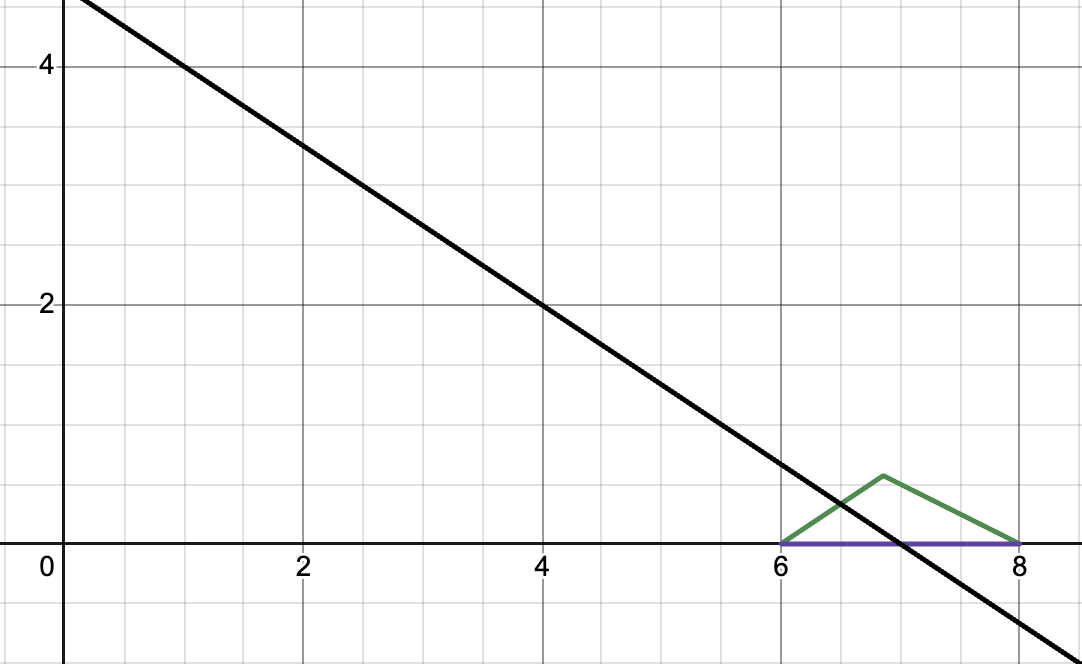
\includegraphics[width=.7\textwidth]{func.png}
\end{center}
Антиградиент
\[-\grad f(x) = (2, 3) = \overline{e}\]
\begin{center}
    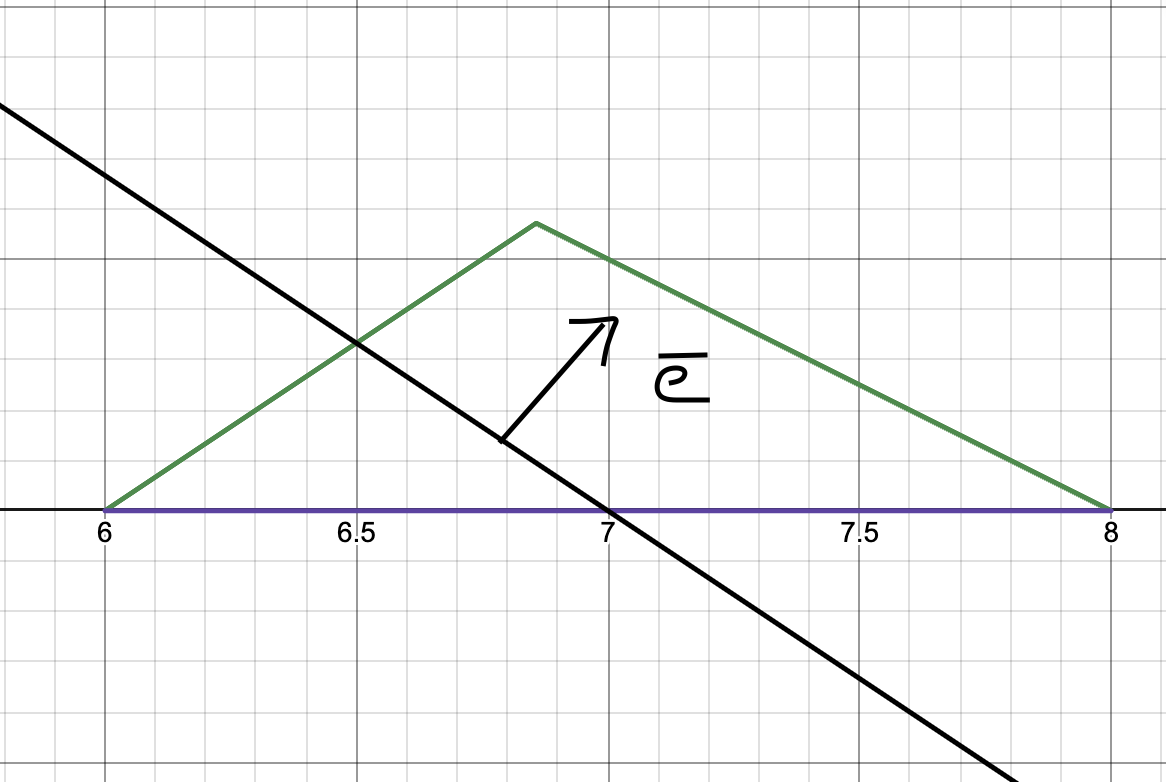
\includegraphics[width=.5\textwidth]{grad.png}
\end{center}
указывает направление убывания функции. 
Совершая параллельный перенос линии уровня вдоль напрвления находим её крайнее положение.
\begin{center}
    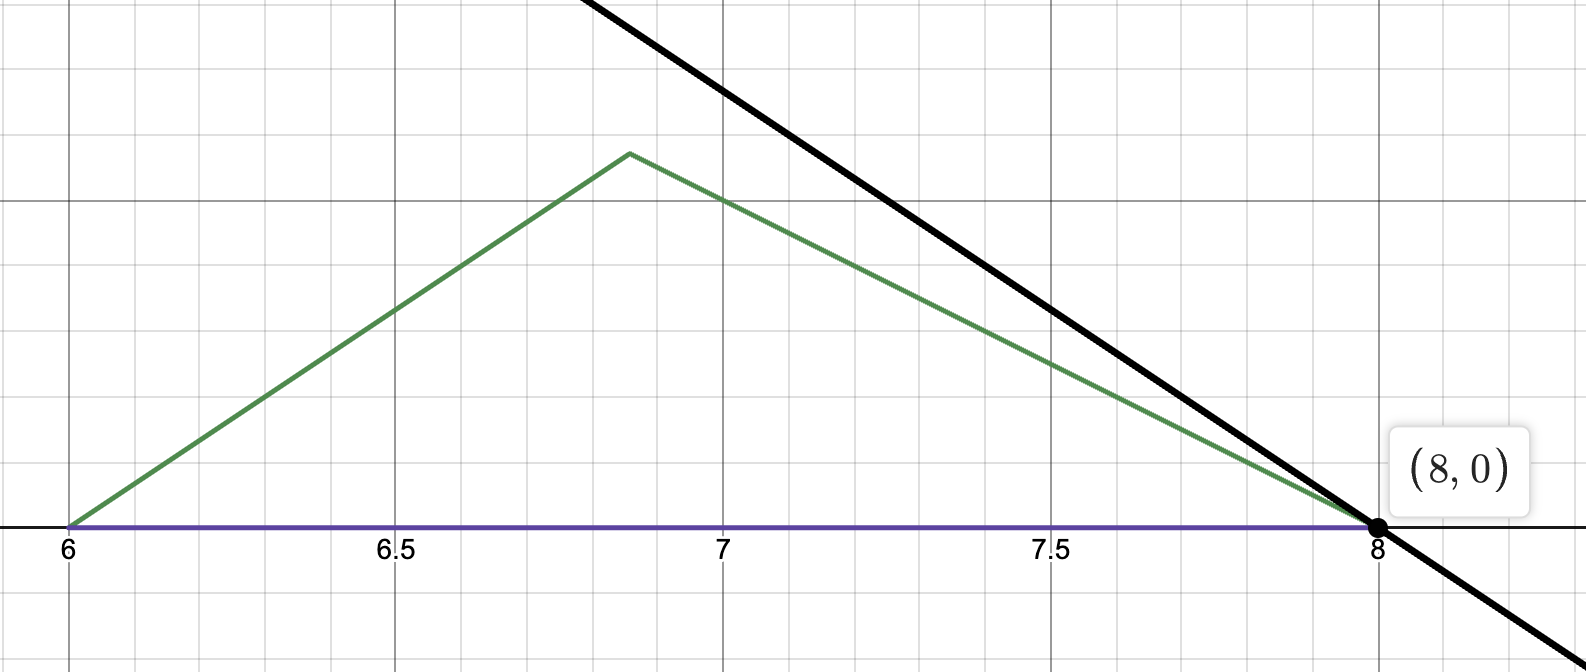
\includegraphics[width=.5\textwidth]{min.png}
\end{center}
В этом положении прямая проходит через вершину с координатами (8, 0).
Поэтому целевая функция f(x) принимает единственное значение в точке x = (8, 0).
\[f^* = -2\cdot 8 - 3\cdot 0 = -16\]

\section*{Задание 2}
Даны матрица А и векторы c и b. Решить каноническую задачу линейного программирования
\[f(x) = cx \ -> max\]
при ограничениях
\[Ax = b,\ x\geq 0\]
с помощью симплекс-метода.
\\ \\
\[c = (0, 1, -6, 1, -3),\ b = (9, 14, 3)\]
\[A = \begin{pmatrix}
    6&1&1&2&1\\
    -1&0&-1&7&8\\
    1&0&2&1&1
\end{pmatrix}\]
Перепишем в удобный вид
\[f(x) = x_2-6x_3+x_4-3x_5\]
\[\begin{cases}
    6x_1+x_2+x_3+2x_4+x_5 = 9\\
    -x_1-x_3+7x_4+8x_5 = 14\\
    x_1+2x_3+x_4+x_5 = 3\\
    x_i \geq 0,\ x_i = 1, ..., 5
\end{cases}\]
Ищем начальное базисное решение:
Столбец 2 является частью единичной матрицы. Переменная пусть x2 входит в начальный базис.
\begin{table}[H]
    \centering
    \caption{Начальная симплекс-таблица}
    \begin{tabular}{|c|c|c|c|c|c|c|}
    \hline
        базис & $x_1$ & $x_3$ & $x_4$ & $x_5$ & b \\ \hline
        $x_2$ & 6 & 1 & 2 & 1 & 9 \\
        ? & -1 & -1 & 7 & 8 & 14 \\
        ? & 1 & 2 & 1 & 1 & 3 \\ \hline
    \end{tabular}
\end{table}
В качестве ещё одной базисной переменной берём x1. 

\begin{table}[H]
    \centering
    \caption{Добавление в базис x1}
    \begin{tabular}{|c|c|c|c|c|c|c|}
    \hline
        базис & $x_1$ & $x_3$ & $x_4$ & $x_5$ & b \\ \hline
        $x_2$ & 6	&1	&2	&1&	9 \\
        $x_1$ & -1&	-3&	7	&8&	14 \\
        ? & 1	&2	&1&	1&	3 \\ \hline
    \end{tabular}
\end{table}
Преобразование: Делим строку 2 на -1. Из строк 1, 3 вычитаем строку 2, умноженную на соответствующий элемент в столбце 1.

\begin{table}[H]
    \centering
    \caption{Преобразование для x1}
    \begin{tabular}{|c|c|c|c|c|c|c|}
    \hline
        базис  & $x_3$ & $x_4$ & $x_5$ & b \\ \hline
        $x_2$	&	-5	&44&	49&	93 \\
        $x_1$ &	1	&-7	&-8	&-14 \\
        $?$  		&1&	8	&9	&17 \\ \hline
    \end{tabular}
\end{table}

В качестве ещё одной базисной переменной берём x3.
\begin{table}[H]
    \centering
    \caption{Добавление в базис x3}
    \begin{tabular}{|c|c|c|c|c|c|c|}
    \hline
    базис  & $x_3$ & $x_4$ & $x_5$ & b \\ \hline
    $x_2$	&	-5	&44&	49&	93 \\
    $x_1$ &	1	&-7	&-8	&-14 \\
    $x_3$  		&1&	8	&9	&17 \\ \hline
    \end{tabular}
\end{table}

Преобразование: Делим строку 3 на -1. Из строк 1, 2 вычитаем строку 3, умноженную на соответствующий элемент в столбце 3.

\begin{table}[H]
    \centering
    \caption{Преобразование для x3}
    \begin{tabular}{|c|c|c|c|c|c|c|}
    \hline
        базис  & $x_4$ & $x_5$ & b \\ \hline
        $x_2$ 	&84&	94	&178 \\
        $x_1$ 	&-15	&-17&	-31 \\
        $x_3$  	&8	&9	&17 \\ \hline
    \end{tabular}
\end{table}

В столбце b присутствуют отрицательные значения. Максимальное по модулю $|b|_{max}$ = 31 находится в строке 2. 
Максимальный по модулю элемент в 2 строке 17 находится в столбце 5. 
Тогда в качестве базисной переменной x1 берём x5.

Преобразование: Делим строку 2 на -17. Из строк 1, 3 вычитаем строку 2, умноженную на соответствующий элемент в столбце 5.

\begin{table}[H]
    \centering
    \caption{Преобразование для x5}
    \begin{tabular}{|c|c|c|c|c|c|c|}
    \hline
        базис  & $x_1$ & $x_4$ & b \\ \hline
        $x_2$ 	&$\frac{94}{17}$&	$\frac{18}{17}$	&$\frac{112}{17}$ \\
        &&& \\
        $x_5$ 	&-$\frac{1}{17}$	&$\frac{15}{17}$&	$\frac{31}{17}$ \\
        &&& \\
        $x_3$  	&$\frac{9}{17}$	&$\frac{1}{17}$	&$\frac{10}{17}$ \\
        &&& \\ \hline
    \end{tabular}
\end{table}

Восстановим функцию:
\[f(x) = x_2-6x_3+x_4-3x_5\]

\[f(x) = (-\frac{94}{17}x_1 -\frac{18}{17}x_4 +\frac{112}{17} )-6
(-\frac{9}{17}x_1-	\frac{1}{17}x_4+	\frac{10}{17})+x_4
-3(\frac{1}{17}x_1	-\frac{15}{17}x_4+	\frac{31}{17})=
-\frac{43}{17}x_1 + \frac{50}{17}x_4 - \frac{41}{17}\]

Симплекс таблица:

\begin{table}[H]
    \centering
    \caption{Добавление f}
    \begin{tabular}{|c|c|c|c|c|c|c|}
    \hline
        базис  & $x_1$ & $x_4$ & b \\ \hline
        $x_2$ 	&$-\frac{94}{17}$&	$-\frac{18}{17}$	&$\frac{112}{17}$ \\
        &&& \\
        $x_5$ 	&$\frac{1}{17}$	&$-\frac{15}{17}$&	$\frac{31}{17}$ \\
        &&& \\
        $x_3$  	&$-\frac{9}{17}$	&$-\frac{1}{17}$	&$\frac{10}{17}$ \\
        &&& \\
        $f$  	&$-\frac{43}{17}$	&$\frac{50}{17}$	&$- \frac{41}{17}$ \\
        &&& \\ \hline
    \end{tabular}
\end{table}
Критерий оптимальности не выполнен.
\[min\{\frac{112}{18}, \frac{31}{15}, 10\} = \frac{31}{15}\]
Тогда $x_4$ попадает в свободные, а $x_5$ в базисные.
\[x_5 = \frac{1}{17}x_1 - \frac{15}{17}x_4 + \frac{31}{17}\]

\[x_4 = \frac{1}{15}x_1 - \frac{17}{15}x_5 +\frac{31}{15}\]
\[x_2 = - \frac{94}{17}x_1 - \frac{18}{17}(\frac{1}{15}x_1 - \frac{17}{15}x_5 +\frac{31}{15}) +\frac{112}{17} = 
-\frac{28}{5}x_1+\frac{6}{5}x_5 +\frac{22}{5}
\]
\[x_3 = -\frac{9}{17}x_1 -\frac{1}{17}(\frac{1}{15}x_1 - \frac{17}{15}x_5 +\frac{31}{15}) +\frac{10}{17} = 
-\frac{8}{15}x_1 + \frac{1}{15}x_5 +\frac{7}{15}
\]
\[f = (-\frac{28}{5}x_1+\frac{6}{5}x_5 +\frac{22}{5})-6(-\frac{8}{15}x_1 + \frac{1}{15}x_5 +\frac{7}{15})+(\frac{1}{15}x_1 - \frac{17}{15}x_5 +\frac{31}{15})-3x_5 = 
-\frac{7}{3}x_1 - \frac{10}{3}x_5 +\frac{11}{3}\]

\begin{table}[H]
    \centering
    \caption{Формирование нового базиса}
    \begin{tabular}{|c|c|c|c|c|c|c|}
    \hline
        базис   & $x_1$            & $x_5$             & b \\ \hline
        $x_2$ 	&$-\frac{28}{5}$  &$\frac{6}{5}$	&$\frac{22}{5}$ \\
        &&& \\
        $x_4$ 	&$\frac{1}{15}$	   &$- \frac{17}{15}$&	$\frac{31}{15}$ \\
        &&& \\
        $x_3$  	&$-\frac{8}{15}$   &$\frac{6}{5}$	&$\frac{7}{15}$ \\
        &&& \\
        $f$  	&$-\frac{7}{3}$	&$- \frac{10}{3}$	&$\frac{11}{3}$ \\
        &&& \\ \hline
    \end{tabular}
\end{table}
Критерий выполнен, ответ получен. 
\[x_1 = 0,\ x_2 = \frac{22}{5}, \ x_3 = \frac{7}{15},\ x_4 = \frac{31}{15},\ x_5 = 0,\ f = \frac{11}{3}\]



\section*{Задание 3}

Данные:
\[C = (-\frac{1}{3}, -\frac{1}{2}, 0, 0, 0)\]
\[b = (-3, -1 ,-5)\]
\[A = \begin{pmatrix}
    -4&2&0&0&2\\
    2&-4&2&0&0\\
    -2&-2&0&2&0
\end{pmatrix}\]
Прямая задача:
\[max(CX|AX = b^T,\ x\geq 0)\]

\[\begin{cases}
    -4x_1+2x_2+2x_5 = -3\\
    2x_1 -4x_2+2x_3 = -1\\
    -2x_1-2x_2+2x_4 = -5
\end{cases}\]

\[f(x) = -\frac{1}{3}x_1 - \frac{1}{2}x_2\ ->\ max\]
Построим двойственную задачу: 
\[min(b\lambda | A^T \lambda \geq c^T,\ \lambda \geq 0)\]
\[A^T = \begin{pmatrix}
    -4&2&-2\\
    2&-4&-2\\
    0&2&0\\
    0&0&2\\
    2&0&0
\end{pmatrix}\]
Двойственная задача имеет вид:
\[g(\lambda) = -3\lambda_1 - \lambda_2 - 5\lambda_3\ ->\ min\]

\[\begin{cases}
    -4\lambda_1 + 2\lambda_2 -2\lambda_3 \geq -\frac{1}{3}\\
    2\lambda_1 -4\lambda_2 -2\lambda_3 \geq -\frac{1}{2}\\
    2\lambda_2 \geq 0\\
    2\lambda_3 \geq 0\\
    2\lambda_1 \geq 0\\
\end{cases}\ ->\ 
\begin{cases}
    -4\lambda_1 + 2\lambda_2 -2\lambda_3 \geq -\frac{1}{3}\\
    2\lambda_1 -4\lambda_2 -2\lambda_3 \geq -\frac{1}{2}\\
    \lambda_{1, ..., 3} \geq 0\\
\end{cases}
\]
\[min(-3\lambda_1 - \lambda_2 - 5\lambda_3) = - max(3\lambda_1 + \lambda_2 + 5\lambda_3)\]
Приведём к каноническому виду, введя дополнительные перменные $\lambda_4,\ \lambda_5$:
\[
\begin{cases}
    -4\lambda_1 + 2\lambda_2 -2\lambda_3 - \lambda_4 = -\frac{1}{3}\\
    2\lambda_1 -4\lambda_2 -2\lambda_3 - \lambda_5 = -\frac{1}{2}\\
    \lambda_{1, ..., 3} \geq 0\\
\end{cases}
\ ->\ 
\begin{cases}
    4\lambda_1 - 2\lambda_2 + 2\lambda_3 + \lambda_4 = \frac{1}{3}\\
    - 2\lambda_1 + 4\lambda_2 + 2\lambda_3 + \lambda_5 = \frac{1}{2}\\
    \lambda_{1, ..., 3} \geq 0\\
\end{cases}
\]
\[\lambda_4 = -4\lambda_1 + 2\lambda_2 - 2\lambda_3 + \frac{1}{3}\]
\[ \lambda_5 =  2\lambda_1 - 4\lambda_2 - 2\lambda_3 +\frac{1}{2}\]
\[g'(\lambda) = 3\lambda_1 + \lambda_2 + 5\lambda_3\]

\begin{table}[H]
    \centering
    \caption{Построение начальной симплекс таблицы}
    \begin{tabular}{|c|c|c|c|c|}
    \hline
    &$\lambda_1$&$\lambda_2$&$\lambda_3$&$\beta$\\\hline
    $\lambda_4$&-4&2&-2&$\frac{1}{3}$\\
    &&&&\\\hline
    $\lambda_5$&2&-4&-2&$\frac{1}{2}$\\
    &&&&\\\hline
    $g'$&3&1&5&0\\
    &&&&\\\hline
    \end{tabular}
\end{table}
Критерий оптимальности не выполнен 
\[min(\frac{1}{6}, \frac{1}{4}) = \frac{1}{6}\]



 $\lambda_3$ попадает в базисные, а $\lambda_4$ попадает в свободные перменные.
\[\lambda_4 = -4\lambda_1+2\lambda_2-2\lambda_3+\frac{1}{3}\]

\[\lambda_3 = -2\lambda_1+\lambda_2-\frac{1}{2}\lambda_4+\frac{1}{6}\]
\[\lambda_5 = 2\lambda_1-4\lambda_2-2(-2\lambda_1+\lambda_2-\frac{1}{2}\lambda_4+\frac{1}{6}) + \frac{1}{2} = 
6\lambda_1-6\lambda_2+\lambda_4+\frac{1}{6}\]
\[g'(\lambda) = 3\lambda_1 + \lambda_2 + 5(-2\lambda_1+\lambda_2-\frac{1}{2}\lambda_4+\frac{1}{6}) = 
-7\lambda_1+6\lambda_2-\frac{5}{2}\lambda_4+\frac{5}{6}\]

\begin{table}[H]
    \centering
    \caption{Симплекс таблица после смены базиса}
    \begin{tabular}{|c|c|c|c|c|}
    \hline
    &$\lambda_1$&$\lambda_2$&$\lambda_4$&$\beta$\\\hline
    $\lambda_3$&-2&1&$-\frac{1}{2}$&$\frac{1}{6}$\\
    &&&&\\\hline
    $\lambda_5$&6&-6&1&$\frac{1}{6}$\\
    &&&&\\\hline
    $g'$&-7&6&$-\frac{5}{2}$&$\frac{5}{6}$\\
    &&&&\\\hline
    \end{tabular}
\end{table}
Критерий оптимальности не выполнен 
\[min(\frac{1}{36}, -) = \frac{1}{36}\]
$\lambda_2$ попадает в базисные, а $\lambda_5$ попадает в свободные перменные.

\[\lambda_5 = 6\lambda_1-6\lambda_2+\lambda_4+\frac{1}{6}\]

\[\lambda_2 = \lambda_1 +\frac{1}{6}\lambda_4 -\frac{1}{6}\lambda_5+\frac{1}{36}\]

\[\lambda_3 = -2\lambda_1+(\lambda_1 +\frac{1}{6}\lambda_4 -\frac{1}{6}\lambda_5+\frac{1}{36})-\frac{1}{2}\lambda_4+\frac{1}{6}=
-\lambda_1 - \frac{1}{3}\lambda_4 - \frac{1}{6}\lambda_5 + \frac{7}{36}\]

\[g' = -7\lambda_1+6(\lambda_1 +\frac{1}{6}\lambda_4 -\frac{1}{6}\lambda_5+\frac{1}{36})-\frac{5}{2}\lambda_4+\frac{5}{6} = 
-\lambda_1 - \frac{3}{2}\lambda_4 - \lambda_5 +1\]

\begin{table}[H]
    \centering
    \caption{Симплекс таблица после смены базиса}
    \begin{tabular}{|c|c|c|c|c|}
    \hline
               &$\lambda_1$&$\lambda_4$&$\lambda_5$&$\beta$\\\hline
    $\lambda_2$&1&$\frac{1}{6}$&$-\frac{1}{6}$&$\frac{1}{36}$\\
    &&&&\\\hline
    $\lambda_3$&-1&$-\frac{1}{3}$&$-\frac{1}{6}$&$\frac{7}{36}$\\
    &&&&\\\hline
    $g'$&-1&$-\frac{3}{2}$&-1&1\\
    &&&&\\\hline
    \end{tabular}
\end{table}
Критерий выполнен.

\[\lambda_1 = 0;\ \ \lambda_2 = \frac{1}{36};\ \ \lambda_3 = \frac{7}{36};\ \ \lambda_4 = 0;\ \ \lambda_5 = 0 \ \ g(\lambda) = -1\]
\[f(x) = g(\lambda) = -1\]



Перейдём к x.
\[X(A^T\lambda - C) = 0\]
\[A^T\lambda - C =\begin{pmatrix}
    -4&2&-2\\
    2&-4&-2\\
    0&2&0\\
    0&0&2\\
    2&0&0
\end{pmatrix} \cdot
\begin{pmatrix}
    0\\
    \\
    \frac{1}{36}\\
    \\
    \frac{7}{36}\\
\end{pmatrix}-
\begin{pmatrix}
    -\frac{1}{3}\\
    \\
    -0.5\\
    \\
    0\\
    \\
    0\\
    \\
    0\\
\end{pmatrix}
= 
\begin{pmatrix}
    -\frac{1}{3}\\
    \\
    -0.5\\
    \\
    \frac{1}{18}\\
    \\
    \frac{7}{18}\\
    \\
    0\\
\end{pmatrix}-
\begin{pmatrix}
    -\frac{1}{3}\\
    \\
    -0.5\\
    \\
    0\\
    \\
    0\\
    \\
    0\\
\end{pmatrix} =
\begin{pmatrix}
    0\\
    \\
    0\\
    \\
    \frac{1}{18}\\
    \\
    \frac{7}{18}\\
    \\
    0\\
\end{pmatrix}
\]

\[
    AX -B =
    \begin{pmatrix}
        -4&2&0&0&2\\
        2&-4&2&0&0\\
        -2&-2&0&2&0
    \end{pmatrix}
    \cdot 
    X -
    \begin{pmatrix}
        -3\\
        -1\\
        -5
    \end{pmatrix} = 
    \begin{pmatrix}
        -4x_1+2x_2+2x_5+3\\
        2x_1-4x_2+2x_3+1\\
        -2x_1-2x_2+2x_4+5
    \end{pmatrix}
\]
\[\begin{cases}
    \frac{2}{36}x_1 - \frac{4}{36}x_2 +\frac{2}{36}x_3 + \frac{1}{36} = 0\\
    -\frac{14}{36}x_1-\frac{14}{36}x_2+\frac{14}{36}x_4 + \frac{35}{36} = 0\\
    x_3,\ x_4 = 0
\end{cases}\ => \ 
\begin{cases}
    \frac{2}{36}x_1 - \frac{4}{36}x_2 + \frac{1}{36} = 0\\
    -\frac{14}{36}x_1-\frac{14}{36}x_2 + \frac{35}{36} = 0\\
    x_3,\ x_4 = 0
\end{cases}\ =>\ 
\begin{cases}
    x_1 = \frac{3}{2}\\
    x_2 = 1\\
    x_3,\ x_4 = 0
\end{cases}
\]
\[-4x_1+2x_2+2x_5=-3\]
\[x_5 = 2x_1 - x_2 -\frac{3}{2} = 3 -1-\frac{3}{2} = \frac{1}{2}\]
\[f(x) = -\frac{1}{3}\cdot \frac{3}{2} - \frac{1}{2}\cdot 1 = -1\]

\textbf{Ответ:}
\[x_1 = \frac{3}{2};\ x_2 = 1;\ x_3 = 0;\ x_4 = 0;\ x_5 = \frac{1}{2};\ f_{max} = -1\]

\end{document}
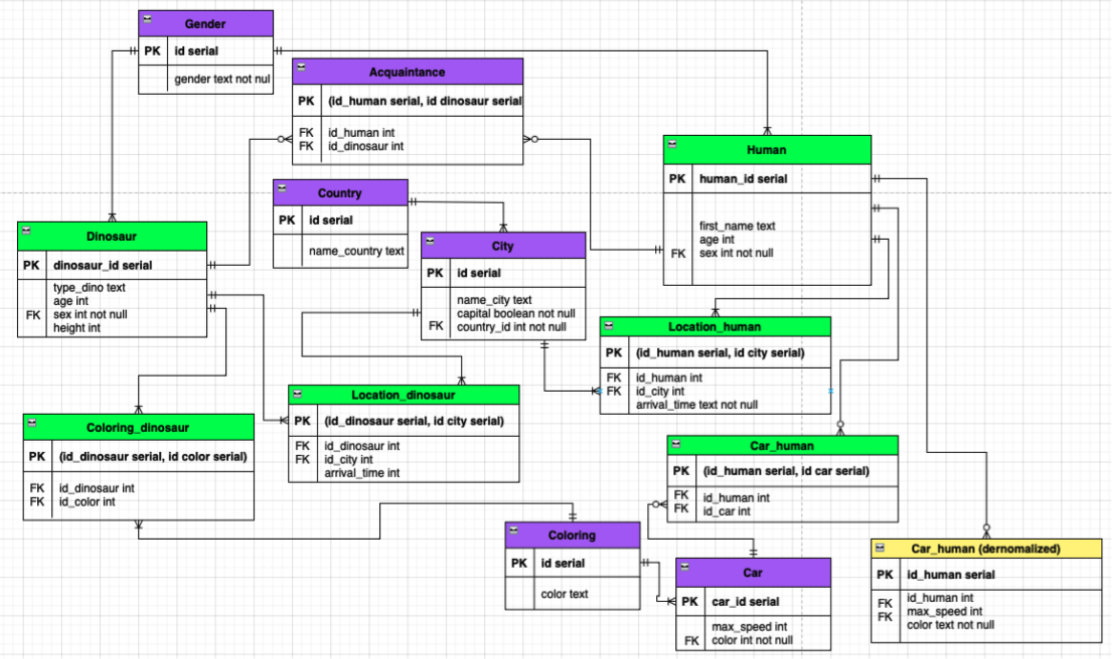
\includegraphics[width=.9\textwidth]{123}


\[f(x) = x_2-6x_3+x_4-3x_5\]

